\documentclass[border=5pt]{standalone}

\usepackage{tikz}
\usetikzlibrary{calc}
%\usepackage{../meccano} adds extra unwanted space!!!

\newcommand{\meccanostrip}[4][000000] % [color]{n}{sep}{prop}
{
 \definecolor{main}{HTML}{#1}
 \draw[main] (0,{{2*#4}})
   -- ++({#2*#3},0) arc(+90:-90:{2*#4})
   -- ++({-#2*#3},0) arc(270:90:{2*#4});
 \foreach \x in {0,1,...,#2}
  \draw[main] (\x*#3,0) circle (#4);
}

\begin{document}
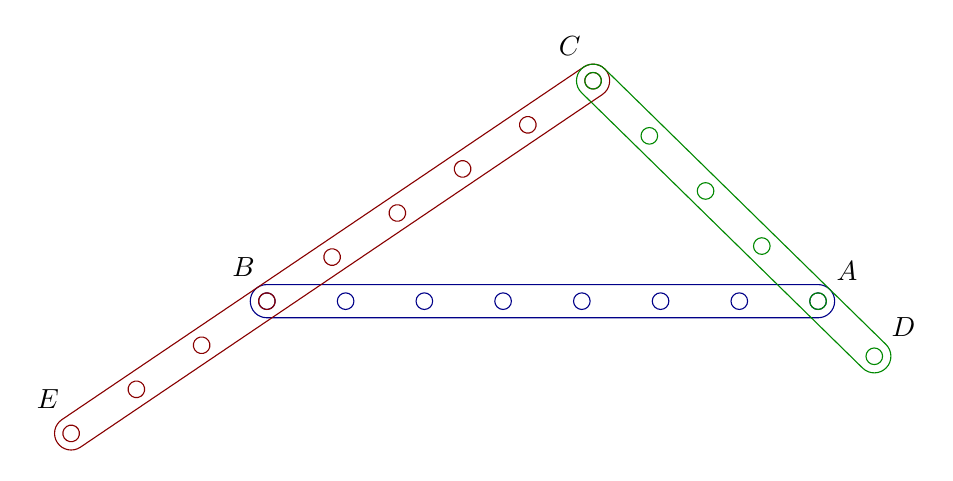
\begin{tikzpicture}

\def\p {3pt}

\def\a{5}
\def\b{4}
\def\c{7}
\def\d{3}
\def\e{1}

\pgfmathsetmacro{\ad}{\a + \d}
\pgfmathsetmacro{\be}{\b + \e}
\pgfmathsetmacro{\cosb}{(\a^2 + \c^2 - \b^2)/(2*\a*\c)}
\pgfmathsetmacro{\cosa}{(\b^2 + \c^2 - \a^2)/(2*\b*\c)}

\begin{scope}
  \meccanostrip[000088]{\c}{1}{\p} % c=BA
   \begin{scope}[rotate={acos(\cosb)},shift={(-\d,0)}]
    \meccanostrip[880000]{\ad}{1}{\p} % a+d=CB+BE
    \path (0,0) ++(90:5*\p) node{$E$};
    \path (\d,0) ++(90:5*\p) node{$B$};
    \path (\a+\d,0) ++(90:5*\p) node{$C$};
   \end{scope}
   \begin{scope}[shift={(\c,0)},rotate=180-acos{\cosa},shift={(-\e,0)}]
    \meccanostrip[008800]{\be}{1}{\p} % b+e=CA+AD
    \path (\e,0) ++(-90:5*\p) node{$A$};
    \path (0,0) ++(-90:5*\p) node{$D$};
   \end{scope}
\end{scope}

\end{tikzpicture}
\end{document}
